\section{\ce{[Cu(dca)_2(4-methoxypyridine)_2]_n}}
\subsection{Synthesis}
2 mmol \ce{Cu(NO_3)_2 * 3 H_2O} (0.48 g), 4 mmol  Na-dicyanamide (0.36 g) and  4 mmol 4-methoxy-pyridine (0.44 g) were dissolved in 45 mL distilled \ce{H_2O}. After stirring for 1 hour at 70$^\circ$C, the mixture was filtered. Then the blue solution was placed in the drying oven ($70^\circ$C) overnight and  cooled down to RT on the next day. A few hours later plate-like  blue crystals were obtained.
Anal. Calculated for \ce{C_{16}H_{14}CuN_{8}O_{2}} (413.90 g/mol) : 46.43\% C; 3.41\% H; 27.07\% N;
Found: 46.45 \% C; 3.44\% H; 27.03 \% N;
IR (ATR, cm$^{-1}$):  2292 (s), 2235 (s), 2169 (s), 1614 (s), 1566 (m), 1510 (m), 1437 (m), 1348 (m), 1303 (s), 1202 (m), 1031 (s), 928 (w), 817 (s), 731 (w), 670 (m), 517 (s)


\begin{figure}[h!]
\centering
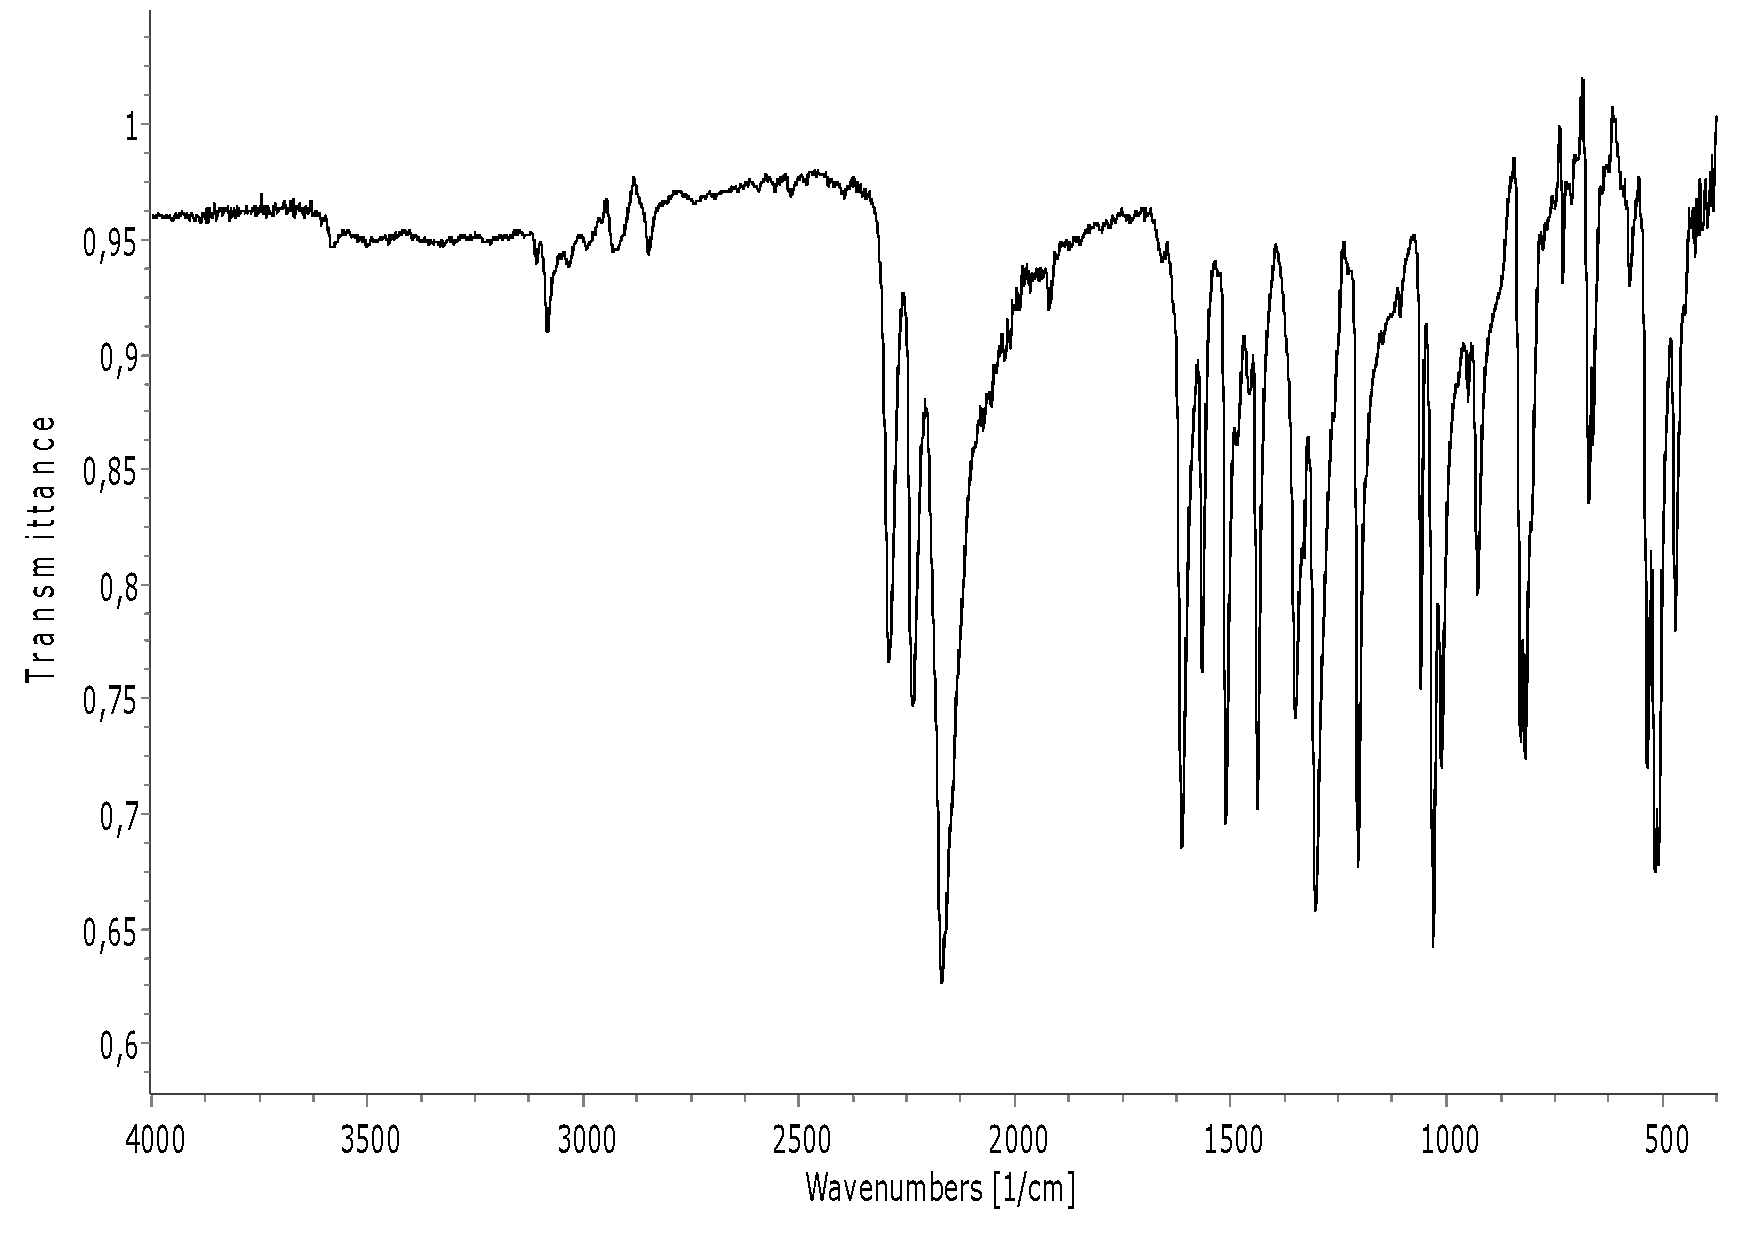
\includegraphics[scale=0.9, width=1\textwidth]{figures/CuD4MOP-IR.pdf}
\caption{IR spectrum of \ce{[Cu(dca)_2(4-MeOpy)_2]_n}}
\end{figure}

\subsection{Structural characterization}

A section of the polymeric chain of \ce{[Cu(dca)_2(4-MeOpy)_2]_n} is depicted in a perspective and a packing view in fig. \ref{fig:CuD4MOP_pv} and fig. \ref{fig:CuD4MOP_packv}. Table \ref{batab:CuD4MOP} shows the bond parameters which have been selected. Two 4-methoxypyridine molecules bind to Cu(1), which is placed on an inversion center. This central metal atom is also connected via the N atoms of four dicyanamide anions. The latter are acting as bis-$\mu$(1,5)-bridging ligands, generating a chain of polyhedra along the b axis of the triclinic unit cell. The \ce{CuN_6} chromophore has an elongated square bipyramidal geometry, with short Cu(1)-N(1) and Cu(1)-N(2) bond distances of 2.0219(9) and 2.0038(10) \AA, respectively, and semi-coordinative Cu(1)-N(4b,c) bond distances of 2.4556(10) \AA. The asymmetric dicyanamide bridges have the following bond parameters: Cu-N-C: 169.61(9) and 148.10(9)$^\circ$; N-C-N: 174.47(12) and 175.12(12)$^\circ$; C-N-C: 119.26(10)$^\circ$; C-N(nitril) 1.1555(15) and 1.1562(15) \AA; C-N(amide): 1.3158(15) and 1.3019(15) \AA. The intra-chain Cu\ce{***}Cu distance of 7.3799(4) \AA  is longer than the shortest inter-chain metal\ce{***}metal separation of 7.0318(4) \AA. 

\renewcommand{\arraystretch}{1.5}
\begin{table}[htpb!]
\centering
\captionabove{Selected bond lengths (\AA) and angles ($^\circ$) for \ce{[Cu(dca)_2(4-MeOpy)_2]_n}; Symmetry codes: (a) -x, -y, 2-z; (b) -x, 1-y, 2-z; (c) x, -1+y, z; (d) x, 1+y, z; (e) -x, -1-y; 2-z; (f) -x, 2-y, 2-z.}
\begin{tabular}{|l|l|l|l|}
\hline
Cu(1)-N(1a) & 2.0219(9) & Cu(1)-N(4b) & 2.4556(10)\\
\hline
Cu(1)-N(2a) & 2.0038(10)& N(3)-C(7) & 1.3158(15)\\
\hline
N(2)-C(7) & 1.1555(15) & N(3)-C(8) & 1.3019(15)\\
\hline
N(4)-C(8) & 1.1562(15) &  & \\
\hline
\hline
N(2)-Cu(1)-N(1a) & 90.33(4) & N(1)-Cu(1)-N(4b) & 90.31(4)\\
\hline
N(4c)-Cu(1)-N(2a) & 92.10(4) & N(2)-Cu(1)-N(2a) & 180.0\\
\hline
Cu(1)-N(2)-C(7) & 169.61(9) & N(2)-C(7)-N(3) & 174.47(12)\\
\hline
Cu(1b)-N(4)-C(8)& 148.10(9) &N(4)-C(8)-N(3) & 175.12(12)\\
\hline
C(7)-N(3)-C(8)& 119.26(10) & &\\
\hline
\end{tabular}
\label{batab:CuD4MOP}
\end{table}


\begin{figure}[!htpb]
\centering
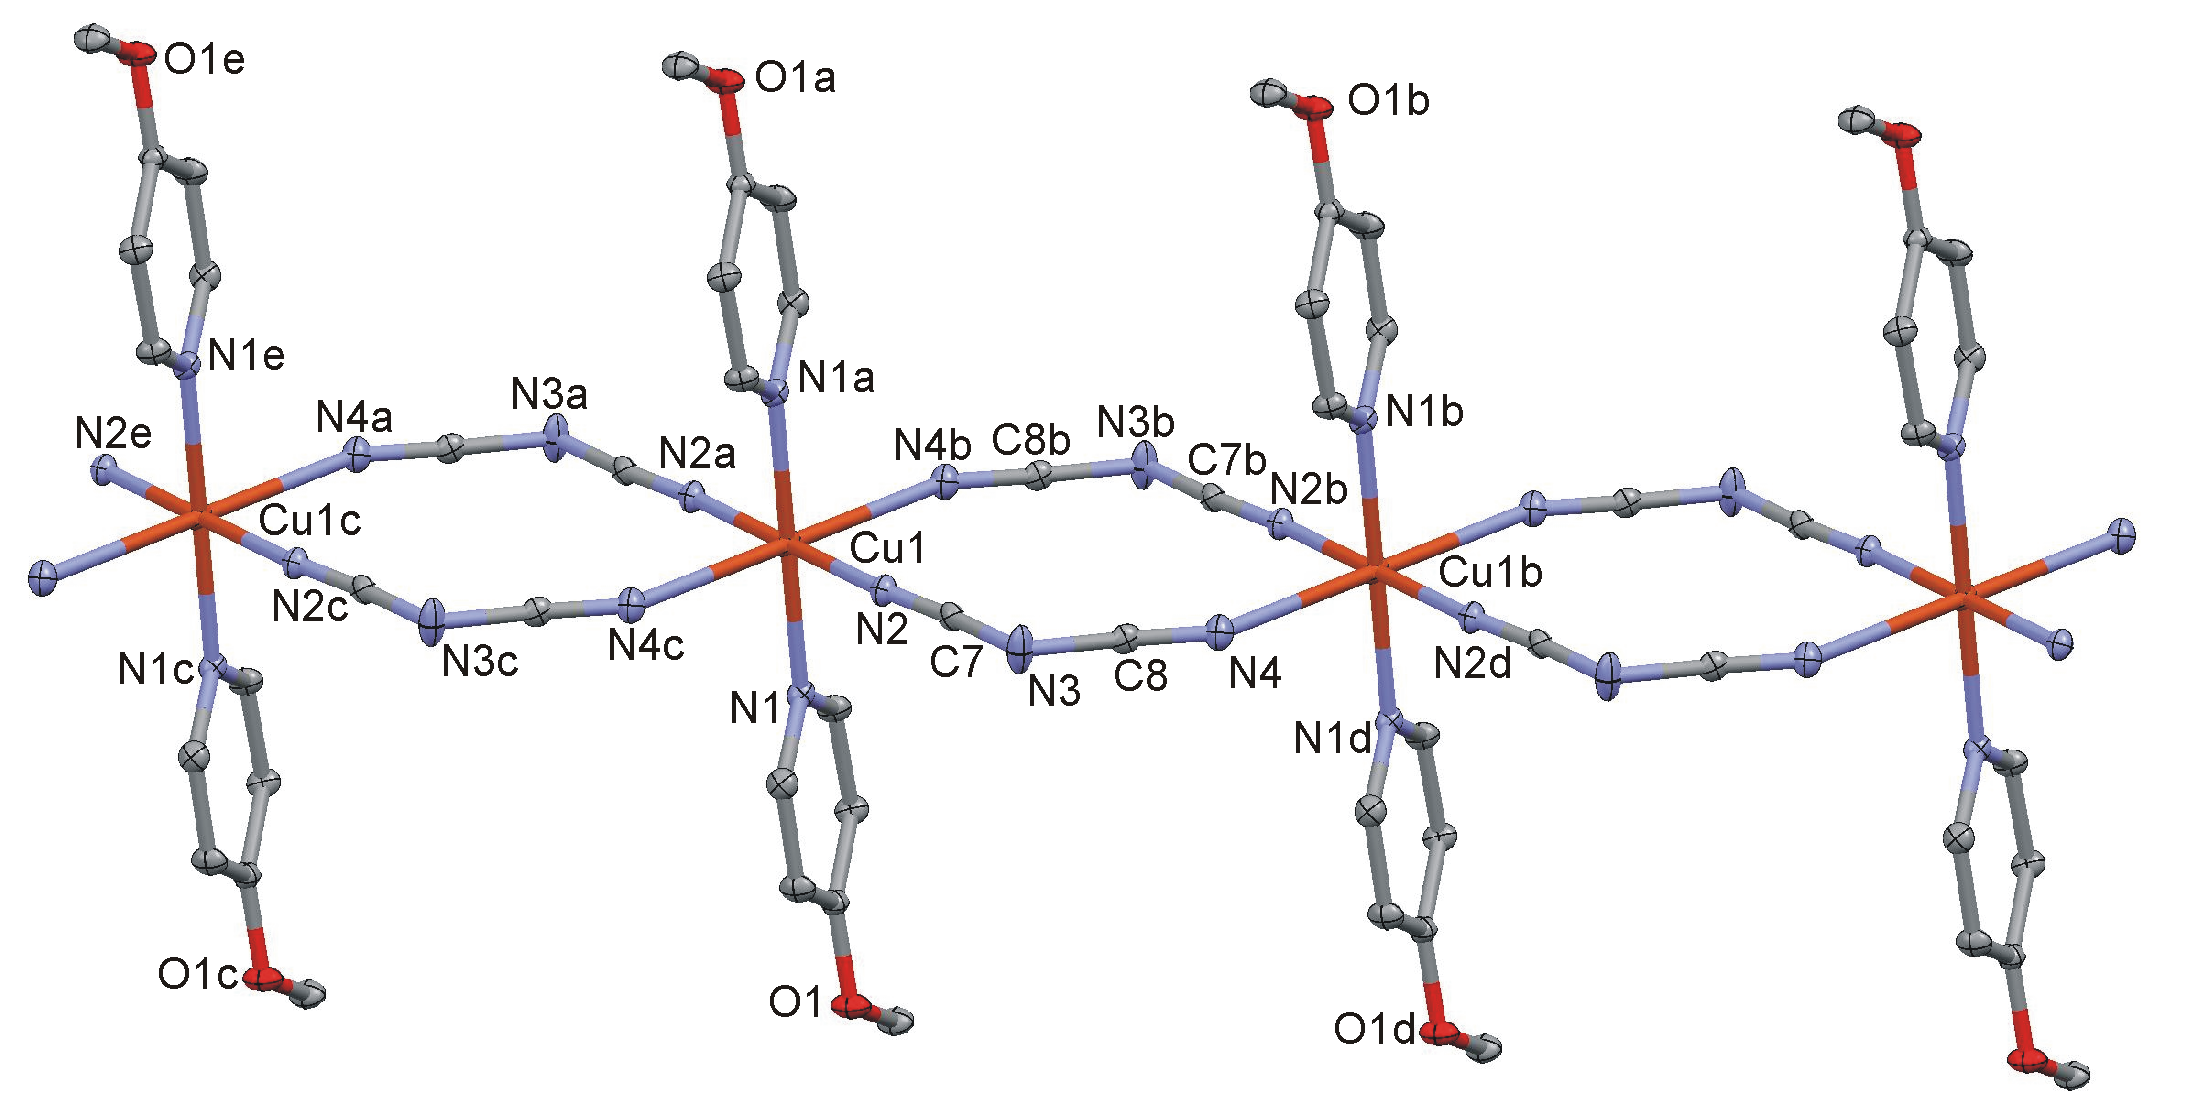
\includegraphics[width=1\textwidth]{figures/cudmop_FIGm11-1.png}
\caption[Perspective view of \ce{[Cu(dca)_2(4-MeOpy)_2]_n}] {Perspective view of a section of the polymeric chain of \ce{[Cu(dca)_2(4-MeOpy)_2]_n} together with the atom numbering scheme. Symmetry codes: (a) -x,-y,2-z; (b) -x,1-y,2-z; (c) x,-1+y,z; (d) x,1+y,z; (e) -x,-1-y,2-z; (f) –x,2-y,2-z.}
\label{fig:CuD4MOP_pv}
\vspace{\floatsep}
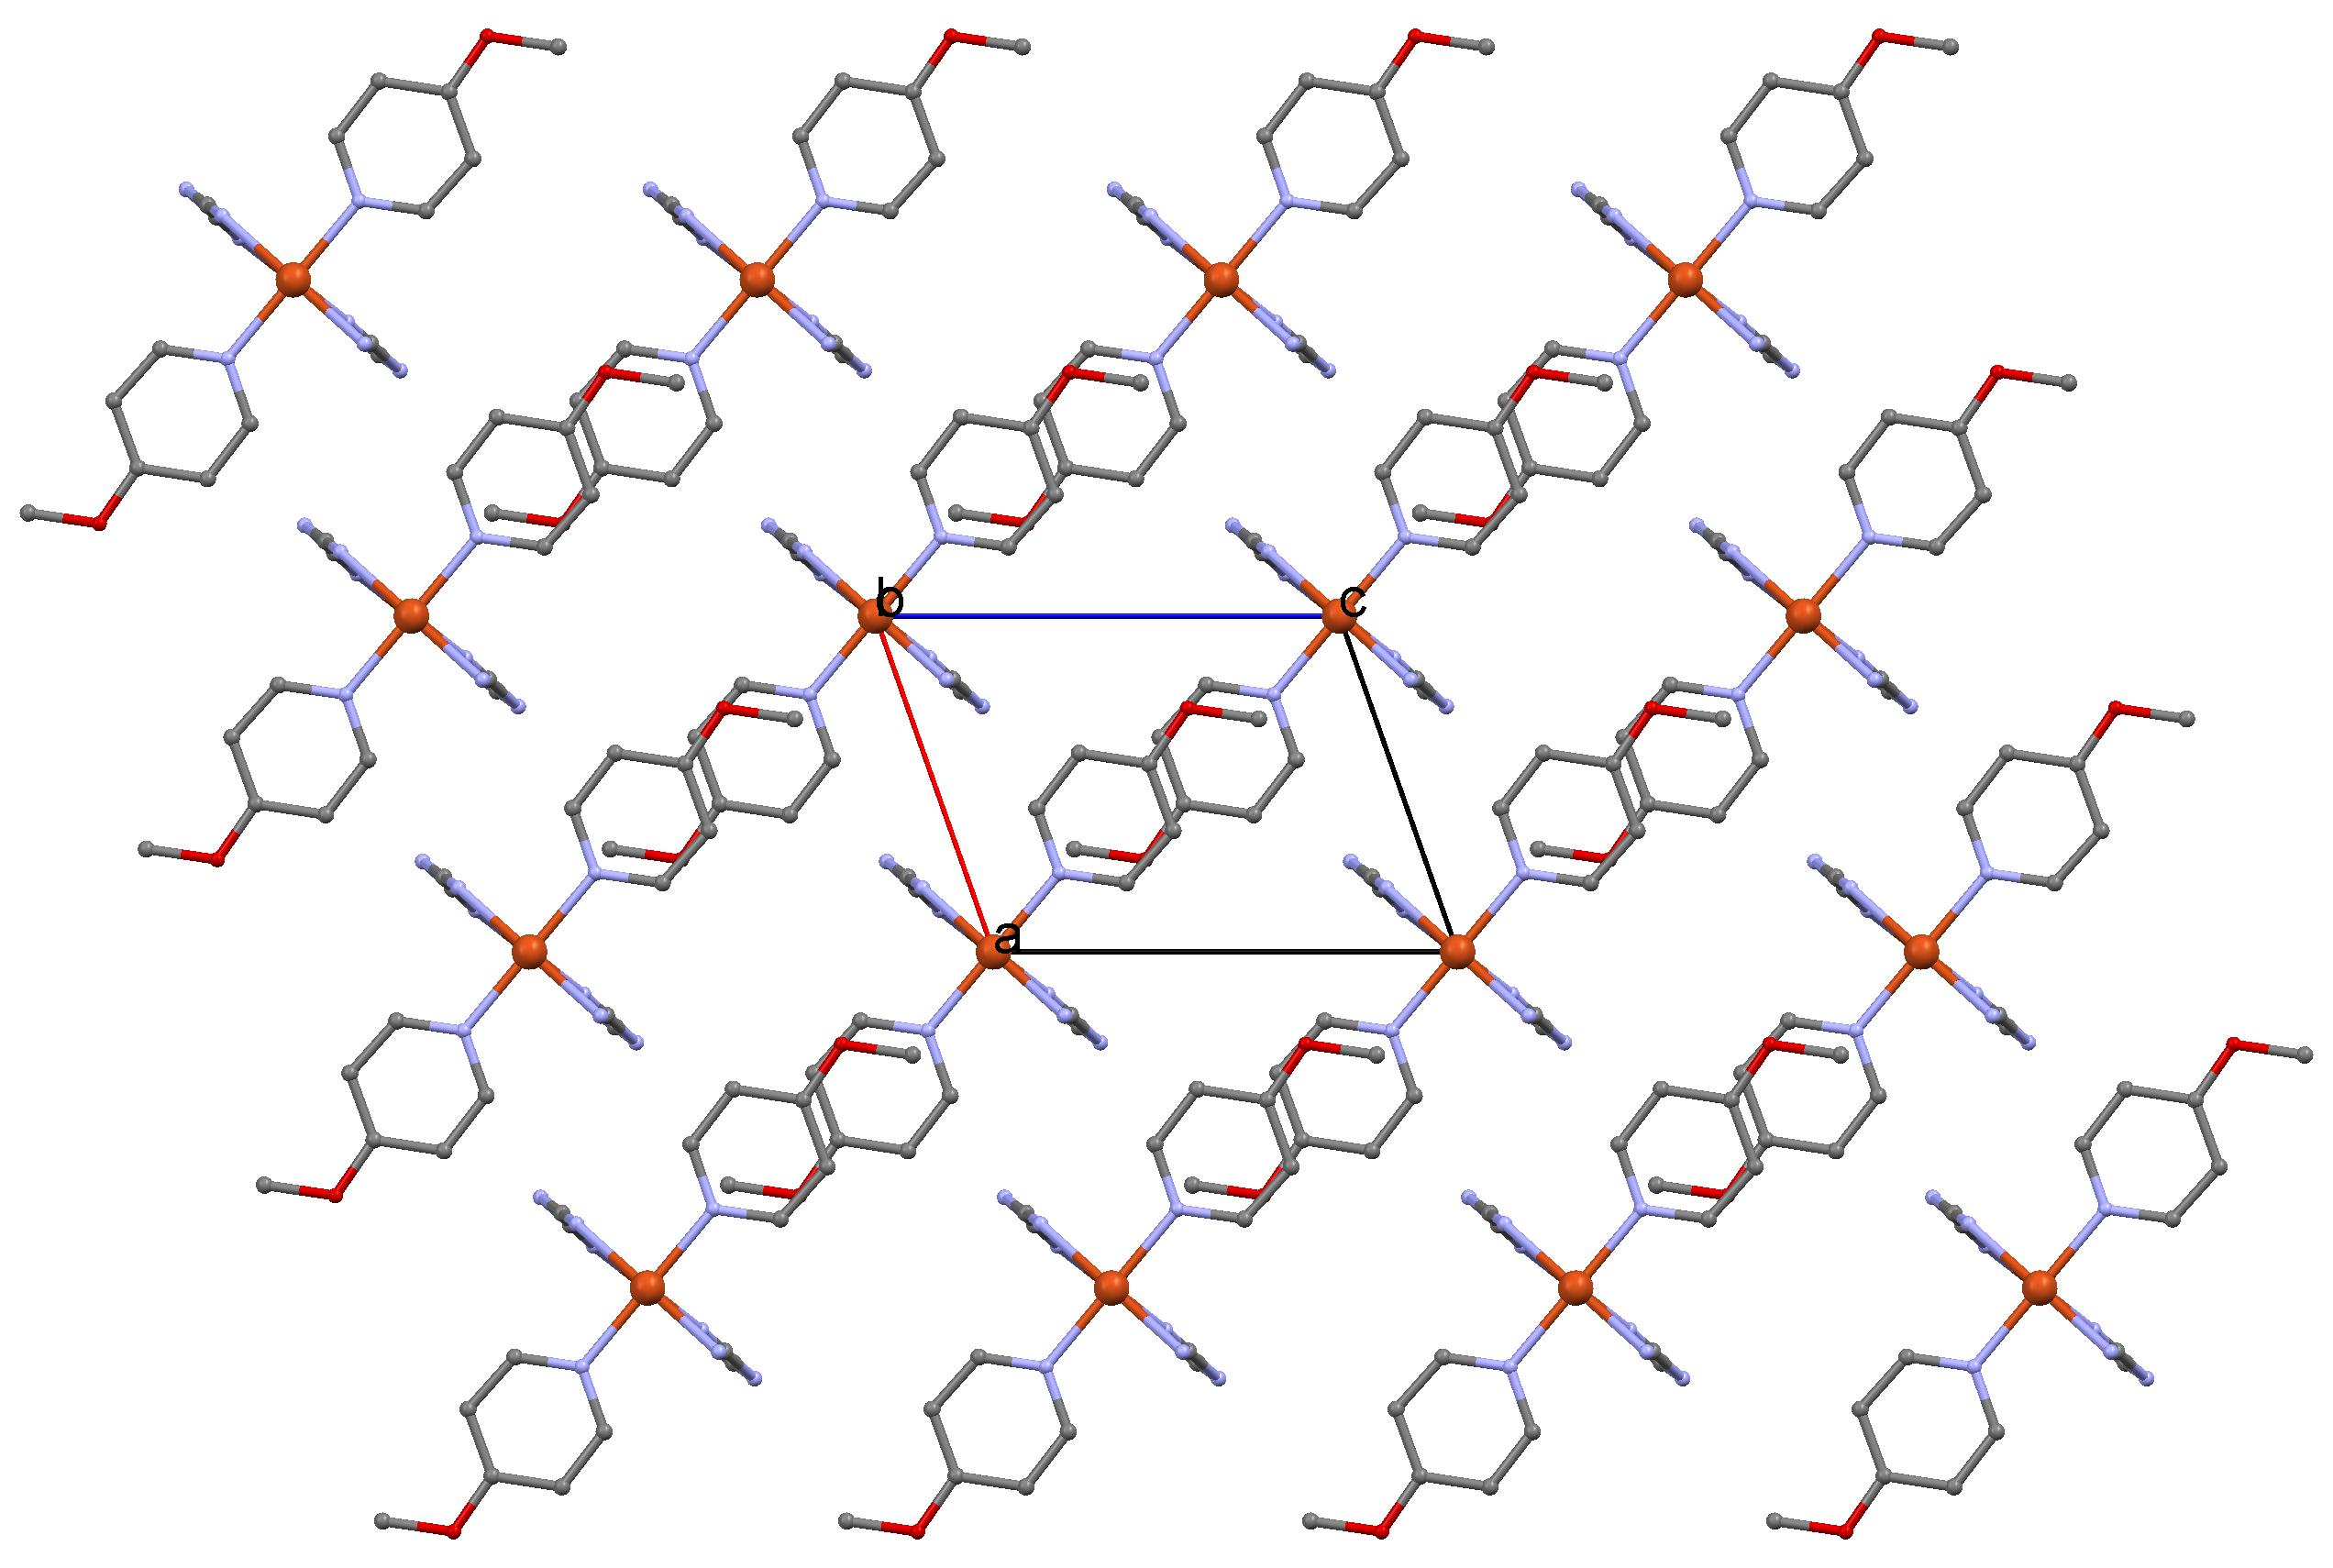
\includegraphics[width=1\textwidth]{figures/cudmop_CB-1.png}
\caption{Packing plot  of \ce{[Cu(dca)_2(4-MeOpy)_2]_n}.}
\label{fig:CuD4MOP_packv}
\end{figure}


\begin{table}
\centering
\captionabove{Crystallographic data and processing parameter of \ce{[Cu(dca)_2(4-MeOpy)_2]n}}
\begin{tabular}{ | l |  l | }
\hline
Empirical formula & \ce{C_{16}H_{14}CuN_{8}O_{2}}\\
\hline
Formula mass & 413.90\\
\hline
System & triclinic\\
\hline
Space group & P-1\\
\hline
a ({\AA}) & 7.0318(3)\\
\hline
b ({\AA}) & 7.3799(3)\\
\hline
c ({\AA}) & 9.7467(5)\\
\hline
$\alpha$ ($^\circ$) & 69.519(2)\\
\hline
$\beta$ ($^\circ$) & 70.257(2)\\
\hline
$\gamma$ ($^\circ$) & 85.367(2)\\
\hline
V (\AA$^{3}) $  & 445.57(4)\\
\hline
Z & 1\\
\hline
T (K) & 100(2)\\
\hline
$\mu$ (mm$^{-1}$) & 1.256\\
\hline
 D$_{calc}$ (Mg/m$^{3}$) & 1.543\\
\hline
Crystal size (mm) & 0.25 x 0.15 x 0.10\\
\hline
$\theta$ max ($^\circ$) & 29.63\\
\hline
Data collected & 24435\\
\hline
Unique refl./ R$_{int}$ & 2514 / 0.0361\\
\hline
Parameters & 125\\
\hline
Goodness-of-Fit on F$^{2}$ & 1.121\\
\hline
R1 / wR2 (all data) & 0.0203 /0.0578\\
\hline
Residual extrema (e/\AA$^{3}$) & 0.42 /-0.43\\
\hline
\end{tabular}

\label{ptab:CuD4MOP}

\end{table}



